\section{The Particle Flow Algorithm}

\begin{figure}
	\centering
	\begin{subfigure}{1\textwidth}
		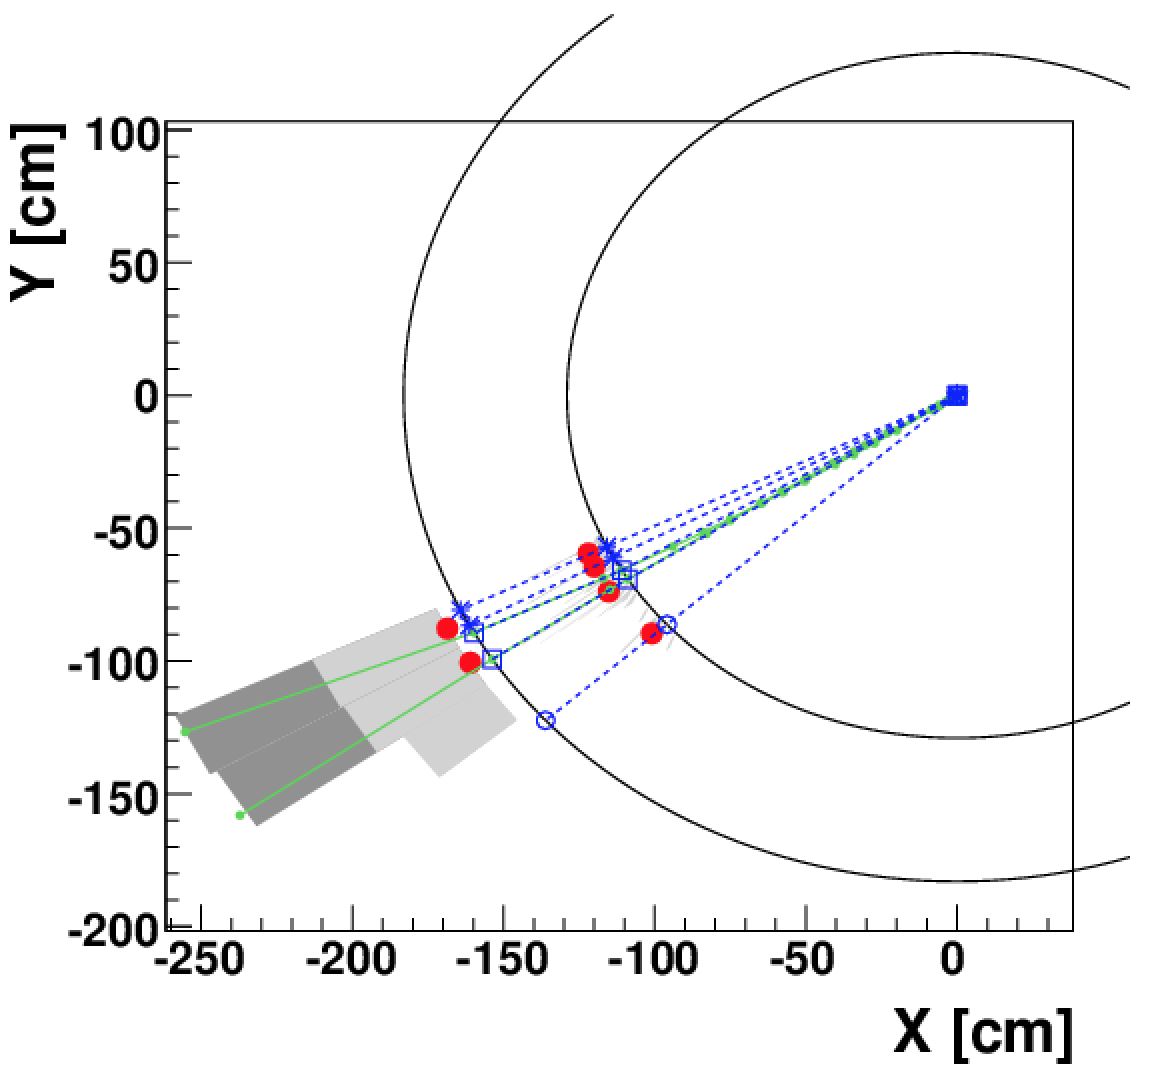
\includegraphics[width=.8\linewidth]{analysis/pics/PF_a.png}
		\caption{The $(x, y)$ view.}
		\label{fig:PF_a}
	\end{subfigure}
	
	\begin{subfigure}{.4\textwidth}
		\centering
		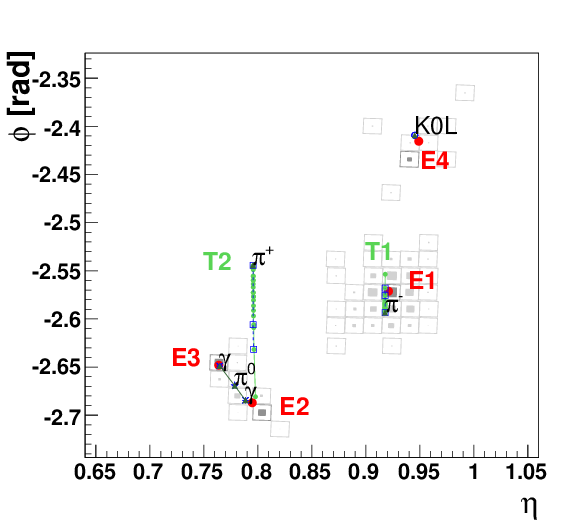
\includegraphics[width=.8\linewidth]{analysis/pics/PF_b.png}
		\caption{The $(\eta,\phi)$ view on ECAL.}
		\label{fig:PF_b}
	\end{subfigure}
		\begin{subfigure}{.4\textwidth}
			\centering
			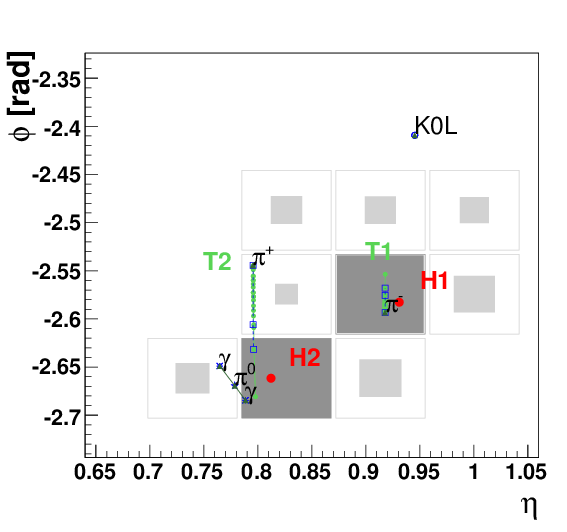
\includegraphics[width=.8\linewidth]{analysis/pics/PF_c.png}
			\caption{The $(\eta,\phi)$ view on HCAL.}
			\label{fig:PF_c}
		\end{subfigure}%
	\caption{An event display of a simple hadronic jet in the $(x, y)$ view (Figure \ref{fig:PF_a}) and in the $(\eta,\phi)$ view, where $\eta$ stands for pseudo-rapidity and $\phi$ for the azimuthal angle, on the ECAL surface (Figure \ref{fig:PF_b}) and the HCAL surface (Figure \ref{fig:PF_c}). (These two surfaces are represented as two circles centred around the interaction point in the first view.) The $K^{0}_{L}$, the $\pi^{-}$ and the two photons from the $\pi^{0}$ decay are detected as four well separated ECAL clusters (Figure \ref{fig:PF_b}). The $\pi^{+}$ leaves no energy in the ECAL. The two charged pions are reconstructed as charged-particle tracks, appearing as vertical solid lines in the $(\eta,\phi)$ views and circular arcs in the $(x, y)$ view. These tracks point towards two HCAL clusters (Figure \ref{fig:PF_c}). In all three views, the cluster positions are represented by dots, the simulated particles by dashed lines, and the position of their impact on the calorimeter surfaces by various open markers.}
	\label{fig:PF_event_display}
\end{figure}

\section {The Tau Lepton reconstruction}

\section {The Jet reconstruction}

